%!TEX root = ../thesis.tex
\newchap{Event classification and signal extraction}\label{sec:signal}
\vspace{-1cm}
\minitoc

\begin{minipage}[H]{\linewidth}
\begin{minipage}{0.35\linewidth}
        \centering
        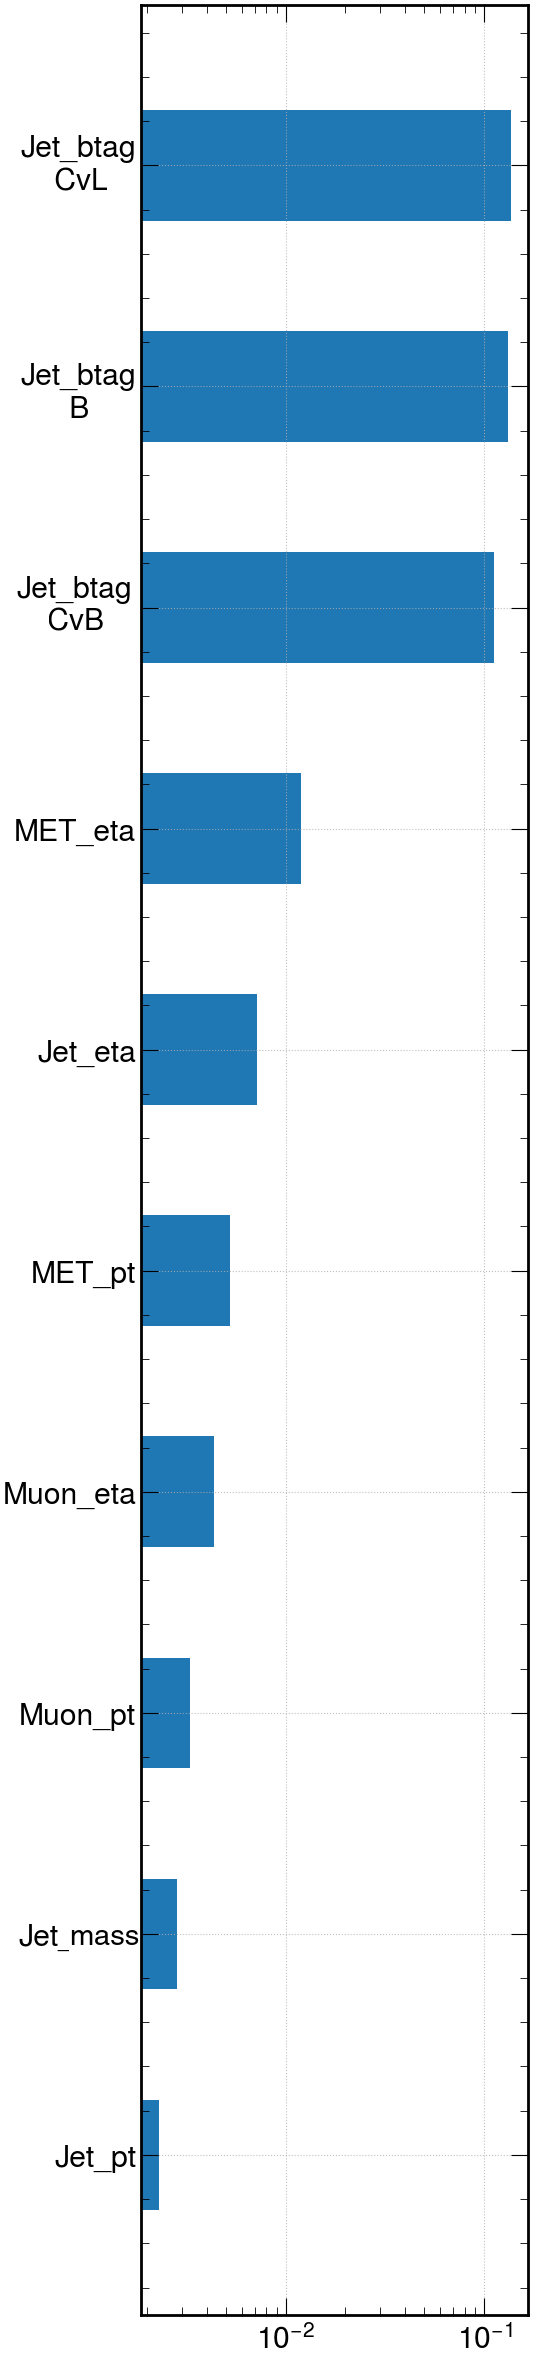
\includegraphics[height=0.92\textheight]{fig//chap08-kin_reco/ranking1D.png}
        \captionof{figure}{Unidimensional feature ranking using the metric $d$ between flattened signal observables and \ttbar semileptonic observables }
        \label{fig:1Drank}
\end{minipage}
\hfill
\begin{minipage}{0.62\linewidth}
\section{Unidimensional feature ranking}
The simplest way to select relevant features that can discriminate the signal from the background is to look at the distribution of different observables, selecting the ones with the most different shapes.\\
The "shape difference" between two histograms can be quantified by the following metric

\begin{equation}
    d=\frac{1}{2}\sum_b \bigg| y_b^{(1)}-y_b^{(2)} \bigg|
\end{equation}
where $y_b^{(i)}$ is the bin height of the b-th bin of the i-th histogram. The histograms are normalized such that their integral is 1.\\
\\
The processes on which the metric $d$ is computed are the signal and the $\ttbar$ semileptonic process, which is the main source of background.\\
All the observables are flattened, \ie all the objects in all the events are collected together in the same histograms, neglecting the structure of the event.\\
The ranking is performed in the Muon channel, after the preselection.\\\\
The result of the unidimensional ranking is shown in \Fig{fig:1Drank} and, without any surprise, the features with the highest separation are the ones related to the b-tagging with $d\sim 0.1$, while the others are one order of magnitude smaller and the latest are practically due only to statistical fluctuations.\\
\\
However, this method is not sufficient because it does not look for correlations between observables. For this reason, multivariate methods like neural networks will be used. \\\\\\\\\\    
\end{minipage}
\end{minipage}
\section{Event classification}
\section{Signal rate extraction}
\subsection{Systematic uncertainties}
\section{Ratio extraction}
\subsection{Systematic uncertainties}